\documentclass[12pt,a4paper]{report}
\usepackage[margin=1.25in]{geometry}
\usepackage[utf8]{inputenc}
\usepackage{graphicx}
\graphicspath{{./images/}}
\usepackage[labelfont=bf]{caption}
\usepackage{booktabs,array}
\usepackage{tocbibind}
\usepackage[toc,page]{appendix}
\usepackage{fancyhdr}
\usepackage{amsmath}
\usepackage{amssymb}
\usepackage[backend=bibtex]{biblatex}
\usepackage{my-notation}
\usepackage{bm}
\usepackage[short]{optidef}
\usepackage{mhchem}
\usepackage{float}
\usepackage{siunitx}
\usepackage{enumitem}
\usepackage{booktabs}
\usepackage{subcaption}
\newtheorem{theorem}{Theorem}[chapter]
\newtheorem{definition}{Defintion}[chapter]
\newtheorem{exmp}{Example}[chapter]

\usepackage[ruled, algochapter, noend, linesnumbered, ruled]{algorithm2e}
\addbibresource{chapters/references.bib}
\pagestyle{fancy}
\fancyhead{}
%\fancyhead[LE,RO]{\textsl{\rightmark}}
\fancyhead[LO,RE]{\textsl{\leftmark}}
\fancyfoot{}
\fancyfoot[C]{\thepage}
\usepackage{algorithm2e}
\usepackage{color}
\usepackage{hyperref}
\hypersetup{
    linktoc=all % 'all' will create links for everything in the TOC
}

\begin{document}
%Titlepage
\begin{titlepage}
	\centering
	
\includegraphics[width=0.5\textwidth]{NTNU}\par\vspace{1cm}
	%{\scshape\LARGE Norwegian University of Science and Technology \par}
	\vspace{1cm}
	{\scshape\Large Masters Specialization Project\par}
	\vspace{1.5cm}
	{\huge\bfseries Sensitivity-Based Economic NMPC with a Path-Following Approach in Python\par}
	\vspace{2cm}
	{\Large\itshape Brittany Hall\par}
	\vspace{2cm}
	{\large Department of Chemical Engineering}
	\vfill
	Supervised by\par
	Johannes J{\"a}schke and Eka Suwartadi

	\vfill

	% Bottom of the page
	{\large \today\par}
\end{titlepage}
%
\tableofcontents
%
\chapter{Summary}
%
\chapter{Introduction}
Model predictive control (MPC), along with non-linear model predictive control (NMPC), is an advanced control strategy that involves solving an optimization problem for a set horizon to determine the feedback value of the manipulated variables at each sampling interval.
These two control strategies are traditionally used widely in the chemical industry for processes with large time constants (i.e., slow dynamics).
Due to modern computation capabilities and algorithm development, this type of control has expanded to more types of systems (even fast dynamics).
MPC has a growing interest in both research and industry due to its performance in a variety of processes in addition to its ability to handle constraints, perform optimization and consider economics and nonlinearities of the process \cite{framework}.
The current areas of interest are: development algorithms for rapid optimization, development better modelling strategies, and new alternatives/variations that lead to improved closed-loop performance or reduce the computation time of the optimization problem.
\par
Most industries care about the profitability of the process which is why economic MPC was developed.
This allows for the integration of the economic optimization and the control layer into a single dynamic optimization layer \cite{economic}.
Economic MPC works by adjusting the inputs such that the economic cost of the operation is directly minimized; thus allowing for the optimization of the cost during operation of the plant.
However, nonlinear process models are often used for this style of optimization meaning that a drawback of economic MPC is the requirement of solving large nonlinear optimization problem (NLP) with the NMPC problem at every sample time.
This computation can take a significant amount of time and lead to increasingly worse performance and even instability of the process \cite{economic}.
\par
One idea to reduce the effect of computational delay in NMPC is to use sensitvity-based methods which exploit the fact that the NMPC optimization problems are identical at each sample time with the exception of one changing parameter: the initial state.
Therefore, the full nonlinear optimization problem is no longer solved.
Instead, the sensitivity of the NLP solution at the previously-computed iteration is used to obtain an approximate solution to the new NMPC problem \cite{economic}.
One such method is the advanced-step NMPC (asNMPC) which involves solving the full NLP at every sample time but this solution is computed in advance for a predicted initial state.
When the new state measurement is available from the process, the NLP solution is corrected using a fast sensitivity update to make the solution match the measured state.
\par
In this project, we focused on applying an improved path-following method for correcting the NLP solution within the advanced-step NMPC framework in Python. 
We illustrate how asNMPC with the predictor-corrector path-following algorithm performs in the presence of measurement noise and compare it with an ideal NMPC approach, where the NLP is assumed to be solved instantly.
\label{ch:intro}
%
\chapter{NMPC}
%%%%%%%%%%%%%%%%%%%%%%%%%%%%%%%%%%%%%%%%%%%%%%%%%%%%%%%%%%%%%%%%%%%%
\section{NMPC Problem Formulations}
%%%%%%%%%%%%%%%%%%%%%%%%%%%%%%%%%%%%%%%%%%%%%%%%%%%%%%%%%%%%%%%%%%%%
%%%%%%%%%%%%%%%%%%%%%%%%%%%%%%%%%%%%%%%%%%%%%%%%%%%%%%%%%%%%%%%%%%%%
\subsection{The NMPC Problem}
We consider a nonlinear discrete-time dynamic system expressed as \cite{economic}:
\begin{equation}
	\boldsymbol{x}_{k+1}=f(\boldsymbol{x}_k,\boldsymbol{u}_k)
	\label{eq:nonlin}
\end{equation}
where $\boldsymbol{x}_k\in\mathbb{R}^{n_x}$ denotes the state variable, $\boldsymbol{u}_k\in\mathbb{R}^{n_u}$ is the control input and $f:\mathbb{R}^{n_x}\times\mathbb{R}^{n_u}\rightarrow \mathbb{R}^{n_x}$ is a continuous model function, which calculates the next state $\boldsymbol{x}_{k+1}$ from the previous state $\boldsymbol{x}_k$ and control input $\boldsymbol{u}_k$, where $k\in\mathbb{N}$.
This system will be optimized by a nolinear model predictive controller which solves the problem:
\begin{mini!}|s|[1]
	{\boldsymbol{z}_l,\boldsymbol{v}_l}{\Psi(\boldsymbol{z}_N+\sum_{l=0}^{N-1}\psi(\boldsymbol{z}_l,\boldsymbol{v}_l)}{}{(\mathcal{P}_{NMPC}):}
	\addConstraint{\boldsymbol{z}_{l+1}=f(\boldsymbol{z}_l,\boldsymbol{v}_l), \qquad l=0,\ldots,N-1}{}
	\addConstraint{\boldsymbol{z}_0=\boldsymbol{x}_k}{}
	\addConstraint{(\boldsymbol{z}_l,\boldsymbol{v}_l)\in\mathcal{Z}}{}
	\addConstraint{\boldsymbol{z}_N\in\mathcal{X}_f}{}
\end{mini!}
at each sample time.
Here $\boldsymbol{z}_l\in\mathbb{R}^{n_x}$ is the predicted state variable; $\boldsymbol{v}_l\in\mathbb{R}^{n_u}$ is the predicted control input; and $\boldsymbol{z}_n\in\mathcal{X}_f$ is the final predicted state variable restricted to the terminal region $\mathcal{X}_f\in\mathbb{R}^{n_x}$.
The stage cost is denoted by $\psi:\mathbb{R}^{n_x}\times\mathbb{R}^{n_u}\rightarrow\mathbb{R}$ and the terminal cost by $\Psi:\mathcal{X}_f\rightarrow\mathbb{R}$.
$\mathcal{Z}$ denotes the path constraints where $\mathcal{Z}=\{(\boldsymbol{z},\boldsymbol{v})|q(\boldsymbol{z},\boldsymbol{v})\leq 0\}$, where $q:\mathbb{R}^{n_x}\times\mathbb{R}^{n_u}\rightarrow\mathbb{R}^{n_q}$.
The solution to this problem is denoted as $\{\boldsymbol{x}_0^*,\ldots,\boldsymbol{z}_N^*,\boldsymbol{v}_0^*,\ldots,\boldsymbol{v}_{N-1}^*\}$
\par
The idea is that at sample time $k$, an estimate or measurement of the state $\boldsymbol{x}_k$ is obtained and the problem $\mathcal{P}_{NMPC}$ is solved,
The first part of the optimal control sequence is then the plant input such that $\boldsymbol{u}_k=\boldsymbol{v}_0^*$.
This part of the solution defines an implicit feedback law $\boldsymbol{u}_k=\kappa(\boldsymbol{x}_k)$, and the system evolves according to Equation \ref{eq:nonlin}.
At the next sample time $k+1$, when the measurement of the new state is obtained, the procedure is repeated.
Algorithm 1 summarizes the NMPC algorithm.\\
\begin{algorithm}[H]
 \caption{General NMPC algorithm.}
	\SetAlgoLined
	set $k\leftarrow 0$\\
	\While{MPC is running}{
		\begin{enumerate}
			\item Measure or estimate $x_k$
			\item Assign the initial state: set $\boldsymbol{z}_0=x_k$
			\item Solve the optimization problem $\mathcal{P}_{NMPC}$ to find $\boldsymbol{v_0^*}$.
			\item Assign the plant input $\boldsymbol{u}_k=\boldsymbol{v}_0^*$
			\item Inject $\boldsymbol{u}_k$ to the plant
			\item Set $k\leftarrow k+1$
		\end{enumerate}
		}
\end{algorithm}
%%%%%%%%%%%%%%%%%%%%%%%%%%%%%%%%%%%%%%%%%%%%%%%%%%%%%%%%%%%%%%%%%%%%
%%%%%%%%%%%%%%%%%%%%%%%%%%%%%%%%%%%%%%%%%%%%%%%%%%%%%%%%%%%%%%%%%%%%
\subsection{Ideal NMPC and Advanced-Step NMPC Framework}
To achieve optimal economic performance and good stability properties, the problem shown in $\mathcal{P}_{NMPC}$ needs to be solved instantaneously, allowing the optimal input to be injected into the process without time delay.
This is known as ideal NMPC.
\par
In reality, there will always be some time delay between obtaining the updated values of the states and injecting them into the plant.
The main cause of this delay is the time required to solve the optimization problem $\mathcal{P}_{NMPC}$.
As the process models grow, so to does the computation time.
With sufficiently large systems, this computational delay cannot be neglected.
One approach is the advanced-step NMPC (asNMPC) which is based on the following steps:
\begin{enumerate}
	\item Solve the NMPC problem at time $k$ with a predicted state value of $k+1$
	\item When the measurement $\boldsymbol{x}_{k+1}$ becomes available at time $k+1$, compute an approximation of the NLP solution using fast sensitivity methods
	\item Update $k\leftarrow k+1$, and repeat from Step 1
\end{enumerate}
Different fast sensitivity methods can be used and are discussed further in Section \ref{sec:}.
%%%%%%%%%%%%%%%%%%%%%%%%%%%%%%%%%%%%%%%%%%%%%%%%%%%%%%%%%%%%%%%%%%%%
\section{Sensitivity-Based Path-Following NMPC}
Below we outline sensitivity results and then utilize them in a path-following scheme for obtaining fast approximate solutions to the NLP.
%%%%%%%%%%%%%%%%%%%%%%%%%%%%%%%%%%%%%%%%%%%%%%%%%%%%%%%%%%%%%%%%%%%%
%%%%%%%%%%%%%%%%%%%%%%%%%%%%%%%%%%%%%%%%%%%%%%%%%%%%%%%%%%%%%%%%%%%%
\subsection{Sensitivity Properties of NLP}
The dynamic optimization problem can be written as a generic NLP problem:
\begin{mini!}|s|[1]
	{\mathcal{X}}{F(\boldsymbol{\chi},\boldsymbol{p})}{\label{eq:param_NLP}}{(\mathcal{P}_{NLP}):}
	\addConstraint{c(\boldsymbol{\chi},\boldsymbol{p})=0}{}
	\addConstraint{g(\boldsymbol{\chi},\boldsymbol{p})\leq 0}{}
\end{mini!}
where $\boldsymbol{\chi}\in\mathbb{R}^{n_{\boldsymbol{\chi}}}$ are the decision variables (typically the state variables and the control input) and $\boldsymbol{p}\in\mathbb{R}^{n_p}$ is the parameter (typically the initial state variable).
$F:\mathbb{R}^{n_{\boldsymbol{\chi}}}\times \mathbb{R}^{n_p}\rightarrow\mathbb{R}$  is the scalar objective function, $c:\mathbb{R}^{n_{\boldsymbol{\chi}}}\times \mathbb{R}^{n_p}\rightarrow\mathbb{R}^{n_c}$ denotes the equality constraints, and $g:\mathbb{R}^{n_{\boldsymbol{\chi}}}\times \mathbb{R}^{n_p}\rightarrow\mathbb{R}^{n_g}$ denotes the inequality constraints.
Each instance of the general parameteric NLP shown in Equation \ref{eq:param_NLP} that are solved for each sample time differ only in the parameter $\boldsymbol{p}$.
(See Suwardti et. al. for the Lagrangian and the Karush-Kuhn-Tucker (KKT) conditions \cite{economic}.)
\par
It has been shown that the perturbed NLP can be solved by solving a QP problem of the form \cite{perturb}:
\begin{mini!}
	{\Delta\boldsymbol{\chi}}{\frac{1}{2}\boldsymbol{\chi}^T\nabla_{\boldsymbol{\chi}\boldsymbol{\chi}}^2\Lagrange(\boldsymbol{\chi}^*,\boldsymbol{p}_0,\boldsymbol{\lambda}^*,\boldsymbol{\mu}^*)\Delta\boldsymbol{\chi}+\Delta\boldsymbol{\chi}^T\nabla_{\boldsymbol{p}\boldsymbol{\chi}}^2\Lagrange(\boldsymbol{\chi}^*,\boldsymbol{p}_0,\boldsymbol{\lambda}^*,\boldsymbol{\mu}^*)\Delta \boldsymbol{p}}{}{\label{eq:QP}}
	\addConstraint{\nabla_{\boldsymbol{\chi}} c_i(\boldsymbol{\chi}^*,\boldsymbol{p}_0)^T\Delta\boldsymbol{\chi}+\nabla_{\boldsymbol{p}}c_i(\boldsymbol{\chi}^*,\boldsymbol{p}_0)^T\Delta\boldsymbol{p}=0\qquad}{i=1,\ldots,n_c}
	\addConstraint{\nabla_{\boldsymbol{\chi}} g_j(\boldsymbol{\chi}^*,\boldsymbol{p}_0)^T\Delta\boldsymbol{\chi}+\nabla_{\boldsymbol{p}}g_j(\boldsymbol{\chi}^*,\boldsymbol{p}_0)^T\Delta\boldsymbol{p}=0\qquad}{j\in K_+}
	\addConstraint{\nabla_{\boldsymbol{\chi}} c_i(\boldsymbol{\chi}^*,\boldsymbol{p}_0)^T\Delta\boldsymbol{\chi}+\nabla_{\boldsymbol{p}}c_i(\boldsymbol{\chi}^*,\boldsymbol{p}_0)^T\Delta\boldsymbol{p}\leq 0\qquad}{j\in K_0}
\end{mini!}
where $K_+=\{j\in\mathbb{Z}:\mu_j>0\}$ is the strongly-active set and $K_0=\{j\in\mathbb{Z}:\mu_j=0 \text{ and } g_j(\boldsymbol{\chi}^*,\boldsymbol{p}_0)=0\}$ denotes the weakly active set.
Note that the solution to this QP is the directional derivative of the primal-dual solution of the NLP, it is a predictor step; thus we refer to (\ref{eq:QP}) as a pure-predictor.
\par
It is important to recognize that the QP is only able to produce the optimal solution accurately for small perturbations and cannot be guaranteed to work for larger perturbations.
One way of handling cases like this to divide the perturbation into several smaller intervals and to iteratively use the sensitivity to track the path of optimal solutions.
This is known as a path-following method.
%%%%%%%%%%%%%%%%%%%%%%%%%%%%%%%%%%%%%%%%%%%%%%%%%%%%%%%%%%%%%%%%%%%%
%%%%%%%%%%%%%%%%%%%%%%%%%%%%%%%%%%%%%%%%%%%%%%%%%%%%%%%%%%%%%%%%%%%%
\subsection{Path-Following Based on Sensitivity Properties}
The basic idea of a path-following method is to reach the solution of the problem at a final parameter value $\boldsymbol{p}_f$ by tracing a sequence of solutions for a series of parameter values given by $\boldsymbol{p}(t_k)=(1-t_k)\boldsymbol{p}_0+t_k\boldsymbol{p}_f$ where $0=t_0<t_1<\ldots<t_k<\ldots<t_N=1$.
The new direction is found by evaluating the sensitivity at the current point.
It is common to include a corrector element into the QP that helps improve the ability of this method to find the correct solution.
\par
We approximate \ref{eq:param_NLP} by a QP, linearized with respect to both $\boldsymbol{\chi}$ and $\boldsymbol{p}$, and enforce the equality of the strongly-active constraints.
\begin{mini}
	{\Delta\boldsymbol{\chi}\Delta\boldsymbol{p}}{\frac{1}{2}\Delta\boldsymbol{\chi}^T\nabla_{\boldsymbol{\chi}\boldsymbol{\chi}}^2\Lagrange(\boldsymbol{\chi}^*,\boldsymbol{p}_0,\boldsymbol{\lambda}^*,\boldsymbol{\mu}^*)^T\Delta\boldsymbol{\chi}+\Delta\boldsymbol{\chi}^T\nabla_{\boldsymbol{p}\boldsymbol{\chi}}^2\Lagrange(\boldsymbol{\chi}^*,\boldsymbol{p}_0,\boldsymbol{\lambda}^*,\boldsymbol{\mu}^*)\Delta\boldsymbol{p}+\nabla_{\boldsymbol{p}}F^T\Delta\boldsymbol{\chi}+\nabla_{\boldsymbol{p}}F\Delta\boldsymbol{p}+\frac{1}{2}\Delta\boldsymbol{p}^T\nabla_{\boldsymbol{p}\boldsymbol{p}}\Lagrange(\boldsymbol{\chi}^*,\boldsymbol{p}_0,\boldsymbol{\lambda}^*,\boldsymbol{\mu}^*)\Delta\boldsymbol{p}}{}{}
	\addConstraint{c_i(\boldsymbol{\chi}^*,\boldsymbol{p}_0-\Delta\boldsymbol{p})+\nabla_{\boldsymbol{\chi}}c_i(\boldsymbol{\chi}^*,\boldsymbol{p}_0+\Delta\boldsymbol{p})^T\Delta\boldsymbol{\chi}=0}{\qquad i=1,...n_c}
	\addConstraint{g_j(\boldsymbol{\chi}^*,\boldsymbol{p}_0-\Delta\boldsymbol{p})+\nabla_{\boldsymbol{\chi}}g_j(\boldsymbol{\chi}^*,\boldsymbol{p}_0+\Delta\boldsymbol{p})^T\Delta\boldsymbol{\chi}=0}{\qquad j\in K_+}
	\addConstraint{g_j(\boldsymbol{\chi}^*,\boldsymbol{p}_0-\Delta\boldsymbol{p})+\nabla_{\boldsymbol{\chi}}g_j(\boldsymbol{\chi}^*,\boldsymbol{p}_0+\Delta\boldsymbol{p})^T\Delta\boldsymbol{\chi}\leq0}{\qquad j\in\{1,\ldots,n_g/K_+\}}
\end{mini}
\par
For the NMPC problem $\mathcal{P}_{NMPC}$, the parameter $\boldsymbol{p}$ corresponds to the current ``initial" state ($\boldsymbol{x}_k$).
The cost function is independent of $\boldsymbol{p}$ which means that $\nabla_{\boldsymbol{p}}F=0$.
In addition, the parameter is linear in the constraints so $\nabla_{\boldsymbol{p}}c$ and $\nabla_{\boldsymbol{p}}g$ are constants.
Applying these simplifications we can write the above QP as:
\begin{mini}
	{\Delta\boldsymbol{\chi}}{\frac{1}{2}\Delta\boldsymbol{\chi}^T\nabla_{\boldsymbol{\chi}\boldsymbol{\chi}}\Lagrange(\boldsymbol{\chi}^*,\boldsymbol{p}_0+\Delta\boldsymbol{p},\boldsymbol{\lambda}^*,\boldsymbol{\mu}^*)\Delta\boldsymbol{\chi}+\nabla_{\boldsymbol{\chi}}F^T\Delta\boldsymbol{\chi}}{\label{eq:QP_pc}}{}
	\addConstraint{c_i(\boldsymbol{\chi}^*,\boldsymbol{p}_0-\Delta\boldsymbol{p})+\nabla_{\boldsymbol{\chi}}c_i(\boldsymbol{\chi}^*,\boldsymbol{p}_0)=0}{\qquad i=0,\ldots,n_c}
	\addConstraint{g_j(\boldsymbol{\chi}^*,\boldsymbol{p}_0-\Delta\boldsymbol{p})+\nabla_{\boldsymbol{\chi}}g_j(\boldsymbol{\chi}^*,\boldsymbol{p}_0)=0}{\qquad j\in K_+}
	\addConstraint{g_j(\boldsymbol{\chi}^*,\boldsymbol{p}_0-\Delta\boldsymbol{p})+\nabla_{\boldsymbol{\chi}}g_j(\boldsymbol{\chi}^*,\boldsymbol{p}_0)\leq0}{\qquad j\in\{1,\ldots,n_g\}/K_+}
\end{mini}
The QP formulation shown above is known as the predictor-corrector form.
This QP tries to estimate how the NLP solution changes as the parameter does in the predictor component and refines the estimate, as the corrector, so that the KKT conditions are more closely satisfied at the new parameter.
\par
The predictor-corrector QP is well suited for use in a path-following algorithm.
Recall that we use the parameter equation: $\boldsymbol{p}(t_k)=(1-t_k)\boldsymbol{p}_0+t_k\boldsymbol{p}_f$.
 At each point $\boldsymbol{p}(t_k)$, the QP is solved and the primal-dual solutions are updated as:
\begin{align}
	\boldsymbol{\chi}(t_{k+1})&=\boldsymbol{\chi}+\Delta\boldsymbol{\chi}\\
	\boldsymbol{\lambda}(t_{k+1})&=\Delta\boldsymbol{\lambda}\\
	\boldsymbol{\mu}(t_{k+1})&=\Delta\boldsymbol{\mu}
\end{align}
where $\boldsymbol{\chi}$ is obtained from the primal solution of the QP (\ref{eq:QP_pc}) and where $\Delta\boldsymbol{\lambda}$ and $\Delta\boldsymbol{\mu}$ correspond to the Lagrange multipliers of the QP.
\par
The QP can detect changes in the active set along the path.
If a constraint becomes inactive, the corresponding mulitiplier $\boldsymbol{\mu}_j$ will first become weakly active meaning that it is added to the set $K_0$.
If a new constraint becomes active, the corresponding linearized inequality constraint in the QP will be active and tracked at the next iteration.
\par
The path-following algorithm is summarized with its main steps in Algorithm \ref{alg:path}.
This algorithm is used to find a fast approximation of the optimal NLP solution corresponding to the new available state measurement; this is done by following the optimal solution path from the predicted state to the measured state.\\
\begin{algorithm}[H]
\SetAlgoLined
\KwIn{initial variables from NLP $\boldsymbol{\chi}^*(\boldsymbol{p}_0),\boldsymbol{\lambda}^*(\boldsymbol{p}_0),\boldsymbol{\mu}^*(\boldsymbol{p}_0)$}
 fix stepsize $\Delta t$, and set $N=\frac{1}{\Delta t}$\;
 set initial parameter value $\boldsymbol{p}_0$,\;
 set initial parameter value $\boldsymbol{p}_f$,\;
 set $t=0$\;
 \For{$k\leftarrow 1$ \KwTo $N$}{
  Compute step $\Delta \boldsymbol{p}=\boldsymbol{p}_k-\boldsymbol{p}_{k-1}$\;
  Solve QP problem\;
  \If{QP is feasible}{
   $\boldsymbol{\chi}\leftarrow\boldsymbol{\chi}+\Delta\boldsymbol{\chi}$\;
   Update dual variables appropriately using either the pure-predictor method or the predictor-corrector method\;
   $t\leftarrow t+\Delta t$\;
   $k\leftarrow k+1$\;
   }
  \Else{
  	$\Delta t\leftarrow\alpha_1\Delta t$\;
	$t\leftarrow t-\alpha_1\Delta t$\;}
}
 \caption{Path-following algorithm}
\end{algorithm}
%%%%%%%%%%%%%%%%%%%%%%%%%%%%%%%%%%%%%%%%%%%%%%%%%%%%%%%%%%%%%%%%%%%%
%%%%%%%%%%%%%%%%%%%%%%%%%%%%%%%%%%%%%%%%%%%%%%%%%%%%%%%%%%%%%%%%%%%%
\subsection{Path-Following asNMPC}
As previously mentioned, for asNMPC, at every time step the full NLP is solved for a predicted state and when a new measurement is available, the precomputed NLP solution is updated by tracking the optimal solution curve from the predicted initial state to the new measured state.
We highlight the fact that the solution of the last QP along the path corresponds to the updated NLP solution and only the inputs from the last QP become inputs to the plant.
One unique quality of this method is that strong and weakly active inequality constraints are differentiated between.
Strongly-active inequalities are linearized and included as equality constraints in the QP, but weakly active constraints are linearized and included as inequality constraints in the QP.
This helps to ensure that the true solution path is tracked more accurately, particularly in the case that the full Hessian of the optimization problem is non-convex \cite{economics}.


%
\chapter{Numerical Case Study}
%%%%%%%%%%%%%%%%%%%%%%%%%%%%%%%%%%%%%%%%%%%%%%%%%%%%%%%%%%%%%%%%%%%%%
\section{Process Description}
We now apply the path-following NMPC on a more relevant example, an isothermal reactor and separator process shown in Figure \ref{fig:process}.
	\begin{figure}[H]
		\centering
		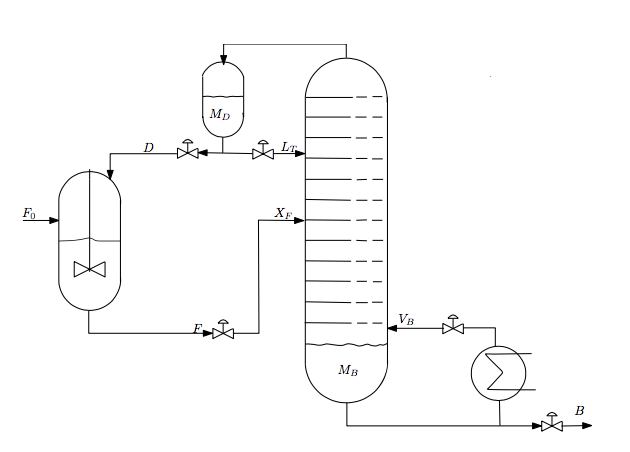
\includegraphics{process}
		\caption{Diagram of a continuously-stirred tank reactor (CSTR) and distillation column.}
		\label{fig:process}
	\end{figure}
The continuously-stirred tank reactor (CSTR) recieves a stream of pure component $\mathcal{A}$ and a recycle stream $\mathcal{R}$ from the distillation column.
A first-order reaction ($\ce{\mathcal{A} -> \mathcal{B}}$) takes place in the CSTR and $\mathcal{B}$ is the desired product. 
The product is then feed with a flow rate $F$ to the distillation column where the unreacted raw material is then separated from the product and recycled to the reactor.
The desired product $\mathcal{B}$ is the bottom product and must have a certain purity.
Table \ref{tab:rxn_kin} summarizes the reaction kinetic parameters for the reactor.
\begin{table}[H]
	\centering
	\caption{Reaction kinetic parameters}
	\begin{tabular}{c c c}
		\toprule[0.3mm]\\
		\textbf{Reaction} & \textbf{Reaction Rate Constant (\si{\per\minute})} & \textbf{Activation Energy (\si{\joule\per\mole})}\\
		\midrule[0.2mm]
		$\ce{\mathcal{A} -> \mathcal{B}}$ & $1\times10^8$ & $6\times10^4$\\
		\bottomrule[0.3mm]
	\end{tabular}
	\label{tab:rxn_kin}
\end{table}
\par
The distillation column model is taken from \cite{model}.
The parameters used for the distillation column are summarized in Table \ref{tab:column}.
\begin{table}[H]
	\centering
	\caption{Distillation column parameters}
	\begin{tabular}{c c}
		\toprule[0.3mm]\\
		\textbf{Parameter} & \textbf{Value}\\
		\midrule[0.2mm]\\
		$\alpha_{AB}$ & 1.5\\
		number of stages & 41\\
		feed stage location & 21\\
		\bottomrule[0.3mm]\\
	\end{tabular}
	\label{tab:column}
\end{table}
The distillation column is comprised of 40 theoretical stages (39 trays and a reboiler) plus a total condenser.
The feed is an equimolar liquid mixture of components $\mathcal{A}$ and $\mathcal{B}$ with a relative volatility of 1.5.
The pressure $P$ is assumed constant due to perfect control of $P$ using $V_T$ as an input.
The reflux and boilup rates are such that we nominally have 99\% purity for reach product ($y_D$ and $x_B$).
The nominal holdup is $M_i^*/F=0.5$ \si{\minute} for all stages, including the reboiler and condenser.
A simple linear relationship $L_i(t)=L_i^*+(M_i(t)-M_i^*)/\tau_L$, where $\tau_L=0.063$ \si{\minute} is used to model the liquid flow dynamics on all trays.
The model uses the following assumptions: binary separation, constant relative volatility, no vapor holdup, one feed and two products, constant molar flows, and a total condenser.
Actuator and measurement dynamics are not included.
\par
The whole model (CSTR and distillation column) has a total of 84 state variables: 82 from the distillation column (mole fractions and liquid holdups from each stage) and two from the CSTR (concentration and holdup).
%%%%%%%%%%%%%%%%%%%%%%%%%%%%%%%%%%%%%%%%%%%%%%%%%%%%%%%%%%%%%%%%%%%%%
%%%%%%%%%%%%%%%%%%%%%%%%%%%%%%%%%%%%%%%%%%%%%%%%%%%%%%%%%%%%%%%%%%%%%
\subsection{Model Equations}
The basic equations used to model the CSTR and distillation column are outlined below.
The notation is outlined in Table \ref{tab:notation}.
\begin{enumerate}[label = \roman*)]
	\item Total balance on stage $i$:
		\begin{equation}
			\frac{dM_i}{dt}=L_{i+1}-L_i+V_{i+1}-V_i
		\end{equation}
	\item Material balance for light component on each stage $i$:
		\begin{equation}
			\frac{d(M_ix_i)}{dt}=L_{i+1}x_{i+1}+V_{i-1}y_{i-1}-L_ix_i-V_iy_i
		\end{equation}
		which also gives the following expression for the derivative of the liquid mole fraction:
		\begin{equation}
			\frac{dx_i}{dt}=\frac{\frac{d(M_ix_i)}{dt}-x_i\frac{dM_i}{dt}}{M_i}
		\end{equation}
	\item Algebraic equations(apply to all stages except condenser, feed and reboiler):
		\begin{itemize}
			\item Vapor-liquid equilibrium
				\begin{equation}
					y_i =\frac{ \alpha x_i}{1+(\alpha-1)x_i}
				\end{equation}
			\item From assumption of constant molar flows and no vapor dynamics (except if feed is partially vaporized):
				\begin{equation}
					V_i=V_{i-1}
				\end{equation}
			\item Linearized liquid flow:
				\begin{equation}
					L_i= L0_i+\frac{(M_i-M0)}{\tau_l}+(V-V_0)_{i-1}
				\end{equation}
				where $L0_i$ \si{\kilo\mole\per\minute} and $M0_i$ \si{\kilo\mole} are the nominal values for the liquid flow and holdup on stage $i$.
		\end{itemize}
	\item Feed stage ($i = NF$):
		\begin{align}
			\frac{dM_i}{dt}&=L_{i+1} -L_i+V_{i-1}-V_i+F\\
			\frac{d(M_ix_i)}{dt}&= L_{i+1}x_{i+1}+V_{i-1}y_{i-1}-L_ix_i-V-iy_i+Fz_F
		\end{align}
	\item Total condenser ($i = NT$):
		\begin{align}
			\frac{dM_i}{dt}&=V_{i-1}-L_i-D\\
			\frac{d(M_ix_i)}{dt}&=V_{i-1}y_{i-1}-L_ix_i-Dx_i
		\end{align}
	\item Reboiler ($i=1$):
		\begin{align}
			M_i&=M_B\\
			V_i&=V_B=V\\
			\frac{dM_i}{dt}&=L_{i+1}-V_i-B\\
			\frac{d(M_ix_i)}{dt}&=L_{i+1}x_{i+1}-V_iy_i-Bx_i
		\end{align}
\end{enumerate}
%%%%%%%%%%%%%%%%%%%%%%%%%%%%%%%%%%%%%%%%%%%%%%%%%%%%%%%%%%%%%%%%%%%%%
%%%%%%%%%%%%%%%%%%%%%%%%%%%%%%%%%%%%%%%%%%%%%%%%%%%%%%%%%%%%%%%%%%%%%
\subsection{Column data}
As mentioned above, the column has 41 stages including the reboiler and total condenser with the feed stage located at stage 21.
The nominal steady state conditions for this column are summarized in Table \ref{tab: column_data}.
\begin{table}[H]
	\centering
	\caption{Column data}
	\begin{tabular}{c c}
		\toprule[0.5mm]\\
		\textbf{Parameter} & \textbf{Value}\\
		\midrule[0.5mm]\\
		Feed rate $F$ & 1 [\si{\kilo\mole\per\minute}]\\
		Feed composition $z_F$ & 0.5 [mole fraction unit]\\
		Feed liquid fraction $q_F$ & 1 [saturated liquid]\\
		Reflux flow $L_T$ & 2.706 [\si{\kilo\mole\per\minute}]\\
		Boilup $V$ & 3.206 [\si{\kilo\mole\per\minute}]\\
		Liquid holdup $M0$ & 0.5 [\si{\kilo\mole}]\\
		Time constant for liquid dynamics $\tau_l$ & 0.063 [\si{\minute}]\\
		$\lambda$ & 0 \\
		Distillate $D$ & 0.5 [\si{\kilo\mole\per\minute}]\\
		Distillate composition $y_D=x_{NT}$ & 0.99 [mole fraction units]\\
		Bottoms $B$ & 0.5 [\si{\kilo\mole\per\minute}]\\
		Bottoms composition $x_B=x_1$ & 0.01 [mole fraction units]\\
		\bottomrule[0.2mm]
	\end{tabular}
	\label{tab:column_data}
\end{table}
This steady state data can easily be recalculated to simulate different columns (number of stages, feed composition, flows, relative volatility, holdups) by using \texttt{col\_model.py} and \texttt{col\_LV.py}. 
%%%%%%%%%%%%%%%%%%%%%%%%%%%%%%%%%%%%%%%%%%%%%%%%%%%%%%%%%%%%%%%%%%%%%
%%%%%%%%%%%%%%%%%%%%%%%%%%%%%%%%%%%%%%%%%%%%%%%%%%%%%%%%%%%%%%%%%%%%%
\subsection{Detailed LV-model}
This model is obtained from model reduction of the detailed 82 state model and only has 5 states.
It includes liquid flow dynamics, composition dynamics, and disturbances.
In this simplified case the inputs are the reflux ($L$) and boilup ($V$) and the controlled outputs are the top and bottom product compositions ($y_D$ and $x_B$).
\par
This simplified model is used to find initial steady state conditions for the distillation column to initialize the remainder of the simulation.
%%%%%%%%%%%%%%%%%%%%%%%%%%%%%%%%%%%%%%%%%%%%%%%%%%%%%%%%%%%%%%%%%%%%%
\section{Objective Function and Constraints}
The economic objective function to be optimized under operation is given by:
	\begin{equation}
		J=p_FF_0+p_VV_B-p_BB
	\end{equation}
where $p_F$ is the feed cost, $p_V$ is the steam cost and $p_B$ is the product price.
The following prices are used in this case study: $p_F=1\, \si{\$\per\kilo\mole}, p_V=0.02\, \si{\$\per\kilo\mole},\text{ and } p_B=2\, \si{\$\per\kilo\mole}$.
The constraints are the concentration of the bottom product ($x_B\leq 0.1$), the liquid holdup at the bottom and the top of the distillation column and in the CSTR ($0.3\leq M_{(B,D,CSTR)}\leq 0.7\,\si{\kilo\mole}$).
The control inputs are the reflux flow ($L_T$), boil-up flow ($V_B$), feed rate to the distillation column ($F$), distillate flow rate ($D$) and bottom product flow rate ($B$).
These control inputs have the following bounds:
\begin{equation}
	\begin{bmatrix} 0.1\\0.1\\0.1\\0.1\\0.1\end{bmatrix}\leq
	\begin{bmatrix} L_T \\ V_B\\F\\D\\B\end{bmatrix}\leq
	\begin{bmatrix} 10\\4.008\\10\\1.0\\1.0\end{bmatrix}
\end{equation}
\par
To solve this problem we must first run a steady-state optimization; we select a feed rate $F_0=0.3\, \si{\kilo\mole\per\minute}$.
This gives optimal values for control inputs and state variables at this feed rate.
The optimal steady state input values are found to be $\boldsymbol{u}_{ss}=\begin{bmatrix}1.18 & 1.92 & 1.03 & 0.74 & 0.29\end{bmatrix}^T$.
\par
The optimal state and control inputs are then used to construct a regularization term that is added to the objective function.
Regularization terms are often used in optimization problems  helps to introduce more information to the function to help solve an ill-posed problem or to prevent overfitting.
The regularization term also helps to regulate the different goals of the objective function.
The new objective function for the regularized stage is written as:
\begin{equation}
	J_m = p_FF_0 + p_VV_B-p_BB-p_DD+(\boldsymbol{z}-\boldsymbol{x}_s)^T\boldsymbol{Q}_1(\boldsymbol{z}-\boldsymbol{x}_s)+(\boldsymbol{v}-\boldsymbol{u}_s)^T\boldsymbol{Q}_2(\boldsymbol{v}-\boldsymbol{u}_s)
\end{equation}
The weights ($\boldsymbol{Q}_1$ and $\boldsymbol{Q}_2$) are selected to make the rotated stage cost of the steady state problem strongly convex. 
To find a valid diagonal regularization matrix $Q$ we utilize the Gershgorin property for a matrix which states for a matrix $\boldsymbol{A}=(a_{ij})$:
	\begin{equation}
		a_{ii}-\sum_{i\neq j}|a_{ij}|\leq \mu_i\leq a_{ii}+\sum_{i\neq j} |a_{ij}|
	\end{equation}
where $\mu_i$ are the eigenvalues of $\boldsymbol{A}$\cite{fast}.
This property can be utilized to systematically find the regularization terms such that the rotated stage cost will be strongly convex and thus
a stable economic NMPC controller can be obtained using this method.
For further details on this method see \cite{fast}.
\par
The distillation column is initialized using the steady states values for a feed rate of $F_0 = 0.29$ \si{\kilo\mole\per\minute} meaning that the controller is essentially controlling for a throughput change from $F_0 = 0.29$ \si{\kilo\mole\per\minute} to $F_0 = 0.30$ \si{\kilo\mole\per\minute}.
The simulation is run for 150 MPC iterations with a sample time of 1 minute.
The prediction horizon of the NMPC controller is set to 30 minute.
This results in an NLP with 10,314 optimization variables (\cite{economic}).
To solve the NLP, CasADi with IPOPT is used; for the QPs, we use CasADi with qpoases (\cite{Andersson2013b}).


%
\chapter{Results}
%%%%%%%%%%%%%%%%%%%%%%%%%%%%%%%%%%%%%%%%%%%%%%%%%%%%%%%%%%
\section{Open-Loop Optimization}
We now compare the solutions obtained from the path-following algorithm with the ``true" solution of the optimization problem $\mathcal{P}_{NMPC}$ obtained by solving the full NLP.
%
\chapter{Discussion}
%
\chapter{Conclusion}
%
\printbibliography

\end{document}